%
\documentclass{report}
% PAGE DIMENSIONS
\usepackage{geometry}
\geometry{a4paper,margin=3.5cm}

% PACKAGES
\usepackage{graphicx} %support the \includegraphics command and options
\usepackage{fancyhdr} % Headers/footers (should be set AFTER setting up the page geometry and before hyperref)
\usepackage{color}
\usepackage{eso-pic} %background pictures
\usepackage[latin1]{inputenc}
%\usepackage[danish]{babel}
%\usepackage[T1]{fontenc}
%\usepackage{courier}
\usepackage{csquotes}
\usepackage{booktabs} % for much better looking tables
\usepackage{tabularx}
\usepackage{slashbox}
\usepackage{array} % for better arrays (eg matrices) in maths
\usepackage{paralist} % very flexible & customisable lists (eg. enumerate/itemize, etc.)
\usepackage{verbatim} % adds environment for commenting out blocks of text & for better verbatim
\usepackage{alltt} %improved verbatim
\usepackage{titlesec} %to modify \chapter, \section, etc appearance
\usepackage{hyperref} %til links, email etc - giver ogs bookmarks i pdf filen
%\usepackage{dirtree} %directory trees
\usepackage{subfig} %make it possible to include more than one captioned figure/table in a single float
\usepackage{float} %float positioning etc
\usepackage{amsmath,amsfonts,amssymb,amsthm} %AMS' packages for symbols, theorems etc.
\usepackage{xfrac} %for nicefrac{}{}
\usepackage{wrapfig}
\usepackage{multicol}
\usepackage{footnote}
\usepackage{perpage}
\usepackage{ctable}
\usepackage[intoc]{nomencl} %for abbreviations list
\usepackage{listings} %for source code listings
\usepackage{marginnote} %Margin notes - use \marginnote{}
%\usepackage[textsize=footnotesize]{todonotes} %the ''disable'' option removes notes
\usepackage{url}
\usepackage{multirow}
\usepackage[normalem]{ulem} %underline, and variations thereof
%\usepackage[parfill]{parskip} %Activate to begin paragraphs with an empty line rather than an indent

% Bibliography appearance
\usepackage[style=numeric,natbib=true,sortcites=true,block=space,backend=bibtex8]{biblatex}
\bibliography{content/bibliography}

% marginnote package options
\renewcommand*{\marginfont}{\color{red}\sffamily} %red, sans-serif
\reversemarginpar %margin notes on left side

% makes footnotes in tables possible (perpage package)
\MakePerPage{footnote}
\makesavenoteenv{tabular}

% listings package settings
\lstloadlanguages{Matlab,[ANSI]C++,[Visual]C++}
\lstset{
  basicstyle=\ttfamily\small,
  %aboveskip=12pt,
  %belowskip=12pt,
  %frame=l,
  numbers=left,
  numberstyle=\ttfamily\tiny,
  numbersep=8pt,
  captionpos=b,
  tabsize=4,
  extendedchars=true,
  breaklines=true,
  showspaces=false,
  showtabs=false,
  keywordstyle=\color{blue},
  escapeinside={(*�}{�*)},
  %rangeprefix=,
  %rangesuffix=,
  includerangemarker=false,
  %stringstyle=\color{white}\ttfamily,
  %commentstyle=\color{white} %''cheat'' to hide comments
  xleftmargin=10pt,
  %backgroundcolor=\color{lightgray},
  showstringspaces=false,
  morekeywords={step,impulse,pzmap,bode,freqz}
}
%\renewcommand*\lstlistingname{Code}

% hyperref package settings
\hypersetup{
    unicode=true,          % non-Latin characters in Acrobat�s bookmarks
    pdftoolbar=true,        % show Acrobat�s toolbar?
    pdfmenubar=true,        % show Acrobat�s menu?
    pdffitwindow=false,     % window fit to page when opened
    pdfstartview={FitH},    % fit page to the window Horizontal/Vertical
    pdftitle={TITLE},    % title
    pdfauthor={Alexander Adelholm Brandbyge, Frederik Hagelskj�r, Rudi Hansen, Leon Bonde Larsen, Kent Stark Olsen, Kim Lindberg Schwaner},% author
    pdfsubject={SUBJECT},   % subject of the document
    pdfkeywords={DTMF} {keyword2} {SDU}, % list of keywords
    pdfnewwindow=true,      % links in new window
    colorlinks=false,       % false: boxed links; true: colored links
    linkcolor=red,          % color of internal links
    citecolor=green,        % color of links to bibliography
    filecolor=magenta,      % color of file links
    urlcolor=cyan,           % color of external links
    plainpages=false
}

% Headers and footers
\pagestyle{fancy} % options: empty , plain , fancy
\setlength{\headheight}{15pt}
%\lhead{\nouppercase{\rightmark}}
\lhead{\nouppercase{\leftmark}}
\chead{}
%\rhead{}
\rhead{\nouppercase{\rightmark}}
\lfoot{}
\cfoot{}
\rfoot{\thepage}

\fancypagestyle{plain}{% Using the plain-style to be able number pages, but with an empty header! (using the report document class makes this nearly obsolete)
 \fancyhf{}
 \renewcommand{\headrulewidth}{0pt}
 \fancyfoot[RO]{\thepage}
}

%%% Contents appearance
\usepackage[]{tocbibind} % Put the bibliography in the ToC (Opts: nottoc,notlof,notlot)
\setcounter{tocdepth}{3} % set how many levels the table of contents displays. default=3
\usepackage[titles,subfigure]{tocloft} % Alter the style of the Table of Contents

% \includegraphics default folder
\graphicspath{{content/graphics/}}

% Number by section
%\numberwithin{equation}{section}
%\numberwithin{figure}{section}
%\numberwithin{table}{section}

% Paragraphs (handled by the parskip package currently?)
%\setlength{\parindent}{0pt}
%\setlength{\parskip}{2ex plus 0.5ex minus 0.2ex}

% Float positioning control
\setcounter{topnumber}{2}
\setcounter{bottomnumber}{2}
\setcounter{totalnumber}{3}
\renewcommand{\topfraction}{0.85}
\renewcommand{\bottomfraction}{0.85}
\renewcommand{\textfraction}{0.15}
\renewcommand{\floatpagefraction}{0.4}

% Header colour
\definecolor{FrontpageHeadingColor}{RGB}{5,5,60}%Heading colour definition

% Chapter name formatting
\titleformat
  {\chapter}%command
  [display]%shape
  {\normalfont\huge\bfseries}%format
  {\normalfont\Large\scshape\chaptertitlename\ \huge\thechapter}%label
  {10pt}%sep
  {\Huge}%before

% make nomenclature and change its heading/toc text (see nomencl package)
\makenomenclature
\renewcommand{\nomname}{Abbreviations}
%
%  * Pass this line to MakeIndex:
%    %bm.nlo -s nomencl.ist -o %bm.nls
%
%  * Use \nomenclature{abbr}{discriptive text} to add an entry to the 
%    abbreviations list (best done where the abbreviation first occurs in the text)
%  * Example:
%    \nomenclature{ADHD}{Attention Deficit Hyperactivity Disorder}

\begin{document}
%
% Front page
\pagenumbering{alph} %frontpage numbered with a letter
\begin{titlepage}%
\currentpdfbookmark{Front page}{front_page}%hyperref pdf bookmark
\AddToShipoutPictureBG*{%background picture	
 \put(0,0){
  \parbox[b][\paperheight][b]{\paperwidth}{%\parbox[position][height][inner-pos]{width}{text}
   \vfill
   %\begin{flushright}
   
\includegraphics[width=0.43\paperwidth,trim=110 0 0 0]{sdu_seal.pdf}%trim=l b r t
   %\end{flushright}
   \vspace*{2.9cm}
  }
 }
}
\begin{flushright}

\includegraphics[scale=0.73]{sdu_logo.pdf}
\end{flushright}
\vspace*{2.7cm}
%
%\textsf{\Large{\textbf{Gruppe 1}}}
%
%\vspace*{0.3cm}
\setlength{\extrarowheight}{1.5pt}
\begin{tabular}{@{}l l}
	\textsf{\large{311289}} & \textsf{\large{Alexander Adelholm Brandbyge}}\\
	\textsf{\large{251289}} & \textsf{\large{Frederik Hagelskj�r}}\\
	\textsf{\large{260387}} & \textsf{\large{Rudi Hansen}}\\
	\textsf{\large{150179}} & \textsf{\large{Leon Bonde Larsen}}\\
	\textsf{\large{040282}} & \textsf{\large{Kent Stark Olsen}}\\
	\textsf{\large{160788}} & \textsf{\large{Kim Lindberg Schwaner}}
\end{tabular}
\setlength{\extrarowheight}{0pt}
\vspace*{1.5cm}
\\
\textsf{\Huge{\textbf{\textcolor{FrontpageHeadingColor}{A generic protocol stack}}}}
\vspace*{0.5cm}
\\
\textsf{\Large{\textbf{\textcolor{FrontpageHeadingColor}{DTMF as information carrier}}}}
\vfill
\textsf{\\Faculty of Engineering\\
University of Southern Denmark\\
Niels Bohrs All� 1\\
5230 Odense M\\
Denmark}
\vspace*{10pt}
\\
\textsf{www.sdu.dk/tek\\
+45 6550 7303\\
tek@tek.sdu.dk}
\end{titlepage}%
%
% Abstract (un-numbered chapter)
\pagenumbering{roman} %until main content we use roman page numbering
\chapter*{Abstract}\addcontentsline{toc}{chapter}{Abstract}
This project is based on the given assignment to create a protocol stack which
use DTMF tones as information carriers, furthermore this has to be done through air
by speaker and microphone. The team agreed on pursuing a secondary objective which
was to develop an application programming interface for easy-to-use utilisation of
the protocol stack.

It is natural therefore to use the layers described in the OSI-model to define
the implementation of the protocol stack itself, and for the composition of the report.
Interdisciplinarity is a big concern for this project as networking- and datacommunication
theory is mixed with the basics of, digital signal processing, software development,
and C++ programming skills. Thus, this report will reflect these skills used to analyse given
problem statements and solving them.

Everything points in the direction of accomplishment of the objective as a fairly stable 
protocol stack was implemented, though it is not efficient compared to state of the art
data communication systems which exist today. In time of writing, the application programming
interface is still under development.

The result work as a proof of concept, that DTMF tones can be used as information carriers
when the data is transported in air. The significance of creating this proof have given a
great insight in topics regarding the basics of, networking and data communication,
digital signal processing, software development, and C++ programming.
%
% Preface (un-numbered chapter)
\chapter*{Preface}\addcontentsline{toc}{chapter}{Preface}
Wee

%
% Table of contents, figures, tables, listings and abbreviations
\tableofcontents
\listoffigures
\listoftables
\lstlistoflistings\addcontentsline{toc}{chapter}{Listings}
\printnomenclature[1.5cm]
%
%
% MAIN CONTENT
\clearpage
\pagenumbering{arabic} %''normal'' arabic numbering from here on out
%
%
\chapter{Introduction}
This is an introduction. Is should contain things like..

This project is devised as a part of the B.Sc. Robot Systems Engineering, 3rd term course at the Faculty of Engineering, University of Southern Denmark, Odense autumn 2011. The implicit goal is to obtain knowledge of computer applications for signal handling. The weight will mainly lay at understanding analogue and digital signals, and integrate this handling in computer applications where computer architecture, operating systems, and data communication will enter into as significant competences.

As the DSMI\footnote{The Engineering Education Model of the University of Southern Denmark} model is used as a framework for this particular education, it is required for the students participating in this course to formulate a strategy for solving a assignment in teams.
\section{Requirements}
This project has in many ways an experimental approach, where it is largely up to the students to figure out how to solve this assignment. This is duo to the requirement of building a protocol stack which uses DTMF tones as data carriers. The exact requirements of the assignment are listed below:

\begin{itemize}
\item Computers have to communicate by exchanging sound.
\item DTMF tones have to be used and a protocol stack have to be build.
\item Information have to be exchanged between computers.
\item A distributed application have to be developed in C++.
\item The architecture have to be layered.
\item It is required that the application perform some meaningful task.
\end{itemize}
\section{Report structure}
The report will be split into several chapters which each explain the different areas that have been explored to fulfil the requirements of this assignment. In chapter \ref{chap:general} the general concepts will be discussed. Chapter \ref{chap:physical} will delve at the physical layer, which define the rules of the data transmission itself and how it should handle this data regarding the upper layer. Chapter \ref{chap:dll} will contain an overview of the data link layer, which explains concepts around the frame, flow control, and error control. Chapter \ref{chap:transport} will explain the workings behind the process-to-process communication. The backbone which control the flow of data between layers is explained in chapter \ref{chap:backbone}. Utilisation and concepts of the application programming interface which acts as the easy-to-use feature of the protocol stack is explained in chapter \ref{chap:api}. Chapter \ref{chap:test} will explain about the test tool that have developed to test each layer separately for stability issues. Experiments conducted will be held in chapter \ref{chap:experiments}. A discussion of the process, solutions, and the results takes place in chapter \ref{chap:discussion}. The conclusion will reside in chapter \ref{chap:conclusion}.

Along with this report a CD will be attached, which contain all material produced during this process. The source and the distributed application will be included on the CD as well.
\section{Project members}
This section will serve as an introduction to each of the project group members. It briefly tells which parts of the project, each member has concerned himself with mostly and what role he has been filling. These roles originate from the Belbin team role model. As the project was begun, the group sat down and discussed which roles they would like to try and fill. They were selected out of a wish to learn what a particular role would involve, and not necessarily what each member is best at.

\begin{description}
\item[Alexander] Has primarily been working on the general architecture of the project, and the developement of the backbone class + associated buffers.
\item[Frederik] Was primeraly responsible for testing. Working with the development of a uniform test-program for debugging and performance testing.
\item[Kent]
has been working with the physical layer which is the lowermost layer of the OSI-model. It has demanded for his skills in terms of understanding the basics of, networking and data communication, digital signal processing, software development, and C++ programming. As a team player Kent is still challenged and he still needs to work on handling conflicts with greater dexterity.
\item[Kim] is a slem bandit
\item[Leon] is a slem bandit
\item[Rudi] is a slem bandit
\end{description}
%
\chapter{General concepts}
Introduction..
\begin{itemize}
 \item An overview.
 \item About network layers, OSI model, what does it mean and why split it in to parts like that?
 \item Explain DTMF - what are those?
 \item Naming conventions? Such as, our library is the ''Dtmf library''
\end{itemize}
\section{Architectural goals}
The user-application thread will spend as little as possible execution time in the network library code.
The network library is completely autonomous, and should be able to function with only minimal interaction from the calling application.
The user should not need to consider any extra memory allocation in the use of this library, i.e. message objects should be handled exclusively by the library.

\subsection{Overall system architecture}
The general idea of this library is to have one, maybe two centralized backbone constructs, which are the only parts of the library to have any long term data storage and awareness of the network state. In the case of sending a network message, the data storage can be regarded as an assembly line, where data is taken from one buffer, transformed and put into the next buffer, in order to apply all the necessary packaging that network communication requires, before the ''end data'' is sent to the audio library.

Each transformation will be done through a separate layer object, that has knowledge of how to encode and decode specific data structures.

Therefore the backbone object is more than just an aggregator of data, its primary function will be to monitor each buffer and control, that transformation of data is done in a way that eliminates congestion as much as possible and ensures no data is lost. Since the backbone must be able to operate autonomously, it will be instantiated with its own execution thread.

In order to ensure that the user application spend as little execution time as possible in the network code, the methods to send and receive data, are designed to be little more than to block copy data to and from the user and the network library.

Each of the selected layers of the OSI model, is represented by an object that can encode or decode a sequence of bytes according to its rules. For instance the Data Link Layer can take a sequence of bytes representing a datagram, and encode it to the form of frames.
However each of the different layer representation has no way of controlling when it is being used, no contextual information(i.e. knowledge of any other object in the system), and are therefore considered pure function objects.

Aside of controlling the execution flow, the backbone will also be responsible for any error reporting, and timing in the application. This will ensure high cohesion and low coupling.

\subsubsection{The backbone class}
The backbone class controls the overall flow of the system by repeatedly checking the state of all buffers and deciding witch needs attention, if more than two buffers have accumulated a sufficient amount of data, it is up to the backbone to choose the most urgent of the two buffers to work with.
The end user application, does not decide how the backbone is allocated explicitly, instead, it will be created upon loading the library and instantiating the API layer. This means that the startup of the library implicitly will be part of the facade pattern.
The backbone class is also responsible for creation of the buffers and for handling settings and errors. The sizes of the buffers may be exposed through the API layer, for the end user to explicitly define buffer sizes, but the library should contain good default values, so the user does not need to configure this manually under most circumstances.

To prevent stalling other processes in the user application, the backbone runs in a separate thread. This introduces concurrency problems at the API layer, when the user application wishes to send and retrieve a message, therefore the buffer must be constructed with this in mind.
The same can happen at the PCM I/O layer, but it is not the responsibility of the backbone to handle this.

The method for determining which buffer to work with, is based on the following criteria.
In the case of sending messages, the portAudio(PCM) buffer should never be empty, unless all the other buffers are empty. Otherwise there will be unneccesary gaps in the audio output.
Likewise, in the case of receiving messages, the backbone should aim to empty the portAudio(PCM) buffer, so there are no ''missed''' samples.
The message receiving part, has a higher priority, since a gap in the listening sequence could potentially result in data loss, where a gap in the output would result in a longer data transfer time (but not necessarily lost packages).

Each downstream buffer has an associated maximum threshold value, and each upstream buffer has a minimum value, which indicates the stable of the library. If there are more data than the max. value, or less data then the min. the backbone will prioritize moving data through the buffers which has passed their threshold values. This mechanism will ensure that buffers who fill up faster will get more processing time.

\subsubsection{Facade class}
Any calls from the user goes through the API class and are passed on to the backbone. Data packages to and from the user also passes through the backbone to ensure low coupling. Since this is the only class the user can instantiate, it also has the responsibility of initializing the rest of the library upon creation.
When a user application wishes to send a message, the API will provide a ''message'' data holder, which can be filled and passed back to the API, this removes the need to do memory handling from the user application.
In order to receive messages from other systems, the user must register a callback function, that will be called by the network library when system has received a complete message. The lifetime of this message will be limited to the scope of the callback function.

\subsubsection{The buffer class}
To ensure maximum reuse of code a generalized buffer class is developed. This class provides one buffer for downwards data and one for upwards. Each buffer is a two-dimensional circular buffer provided by the included boost library. The buffer class contains methods for calling the layers and for providing information to the backbone.
By making the buffer two dimensional, it is possible to apply locks to individual sections of the data instead of a complete read/write lock, and thereby vastly increasing insert/delete operations.

Three  buffer objects are instantiated: A package buffer, a datagram buffer and a frame buffer. Each buffer is accessible from both the overlying and the underlying layer. And when a buffer is attended by the backbone it calls the appropriate function in the responsible layer.

\subsubsection{The layer classes}
The three layer classes reads data from a buffer, works on the data and writes it into the next buffer in the chain. Each layer may instantiate temporary internal buffers to store partially processed data between attention. Some of the layers will need to send a message to the layer before it, and when executing an encode or decode function, the layer is given access to both the appropriate send and receive buffers.

\subsubsection{The interface class and portAudio}
The interface class implements its own circular buffer, since portaudio resides in the core memory bla bla


\subsubsection{Overview of the send/receive process}
\begin{description}
\item[Sending Application]
Duty: The application calls the API, providing data and relevant delivery information
Output: Data and destination.
\item[Sending API layer]
Input: Data and destination.
Duty: The API layer encloses the message into a package, adding a header containing info about receiving process.
Output: A package.
\item[Sending session layer]
Input: A package
Duty: The session layer opens, negotiates and maintains the connection. It segmentates the data, adding destination and sender addresses, session ID, flags, total length and sequence number to each datagram.
Output: A datagram
\item[Sending data link layer]
Input: A datagram
Duty: The data link layer segmentates the datagram and encodes each with a header containing sequence number, address, frame type and checksum.
Output: Frames
\item[Sending physical layer]
Input: A frame
Duty: The physical layer translates each four bit sequence into DTMF tone data.
Output: PCM string
\item[Sending sound system interface]
Input: PCM string
Duty: To parse data to the sound system
Output: DTMF tones
\item[Receiver side]
Receiving sound system interface
Input: DTMF tones
Duty: Record sound input into a buffer.
Output: PCM bytes
\item[Physical layer]
Input: PCM bytes
Duty: The physical layer reads the buffered data and interprets any DTMF tone data into four bit sequences. When six tones are received the corresponding 3 byte frame is buffered.
Output: A frame
\item[Data link layer]
Input: Frames
Duty: The data link layer checks the received frame and discards it if errors have occurred. It then gathers the frames, removes the headers and reassembles them into a datagram. If frames are missing, resending is requested from the sending data link layer.
Output: A datagram
\item[Network layer]
Input: A datagram
Duty: Negotiates and maintains the connection. Removes the header and reassemble the data into a package.
Output: A package
\item[API layer]
Input: A package.
Duty: The API layer removes the header and presents the final message to the receiving process.
Output: Data
\item[Application]
Input: Data
Duty: The application interprets and uses the received data
\end{description}
%
\chapter{Design decisions}
%available alternatives, decisions made, theory of operation
%\begin{itemize}
%\item ''our'' layers	
%\item backbone
%\item test class
%\item application to use with our network
%\end{itemize}

To facilitate development, the sound sound network protocol is divided into layers corresponding to those of the OSI model. The functionality of each layer and it's responsibilities will, at first, be descriped seperately in this chapter. yada yada
\nomenclature{API}{Application programming interface}
\section{Application programming interface}
The application programming interface (API) layer is designed with the goal of presenting an easy-to-use interface for the Dtmf library. Threading is used to avoid stalling the front end application when sending and receiving data. 
\subsection{Method description}
\subsubsection*{Public DtmfApi(unsigned char myAddress,bool hasToken, DtmfApiMsgInCallback * callback);}
This is the constructor method of the API class. This method is called when the class is to be used.
When this method is called, two threads are started. One for sending/receiving data and one for user callback. These threads ensure that the end application don't have to wait for the sending a receiving algorithms that needs to be running.

\subsubsection*{Public void makeToken();}
In case the token will get lost in the network, it is possible to manually insert a token with this method. When called the node on which it's called gets the token. Token passing method is documented here ?? (This method might be obsolete, as this is may be handled automatically by DDL)

\subsubsection*{Public DtmfOutMessage newMessage();}
This method is used when sending data. It returns a empty message, and enables the user to fill ind the message data manually. A reference is kept to the DtmfApi, so the message can be send by the build in method DtmfOutMessage::send();

\subsubsection*{Public void sendMessage(unsigned char rcvAddress, char * data, unsigned long dataLength);}
When this method is called with arguments, the message is created internally and send right away.

\subsection{Thread description}
Two threads are spawned when the API layer is initialized. The general idea behind these threads is to avoid interference between the Dtmf lib and user application. The Dtmf needs to constantly monitor the surrounding sounds to be able to reply in time. Using seperate threads avoids user algorithms stalling these important processes.

\subsubsection{Callback thread}
This thread is only used for calling the user specified callback function when data is received. 

\subsubsection{Backbone thread}
The backbone thread is responsible for controlling internal buffers and send/receive logic. This is described in ?? 


\subsection{Usage example}
\subsubsection{Creating instance}
\begin{lstlisting}[float=htb,language={[ANSI]C++},caption={Creating instance example},label=CreatingInstanceEx]
// Declare callback function
void function MyClass::messageInCallback(DtmfInMessage m)
{
    // This function is called everytime data arrives. The incoming message only exist inside this method, so it's recommended to copy all needed information before exiting the function.
    return;
}
int main()
{
unsigned char myAddress = 1; // My address is 1
bool hasToken = true; // When starting I have the token. Only one node should have this flag set. When connection to an already running DTMF network this should be set to false.

DtmfApi *api = new DtmfApi(myAddress, hasToken, &MyClass::messageInCallback);
// DTMF API is now running.
(...)
\end{lstlisting}

\subsubsection{Sending data}
(This example assumes that an instance of API already has been created. See example \ref{CreatingInstanceEx})
The library support two ways of sending a message. Each with different advantages.
First method - the fast way:
\begin{lstlisting}[float=htb,language={[ANSI]C++},caption={Sending data example 1},label=SendingDataEx1]
api->sendMessage(unsigned char rcvAddress, char * data, unsigned long dataLength);
\end{lstlisting}

Second method - building a custom message:
\begin{lstlisting}[float=htb,language={[ANSI]C++},caption={Sending data example 2},label=SendingDataEx2]
DtmfOutMessage message = api->newMessage(); // Create an empty message
message.setData(char * data, unsigned long startAdress, unsigned long dataLength);
message.send();
\end{lstlisting}

\subsubsection{Receiving data}
(This example assumes that an instance of API already has been created. See example \ref{CreatingInstanceEx})
\begin{lstlisting}[float=htb,language={[ANSI]C++},caption={Receiving data example},label=ReceivingDataEx]
void function MyClass::messageInCallback(DtmfInMessage m)
{
    // This method is called when new data arrives.
    // Fetch data from DTMF class to local memory (Assuming we have a dataContainer available in the MyClass)
    m.getData(this->dataContainer*, 0, m.getMessageLength());
    return;
}
\end{lstlisting}

\section{Physical Layer}

	\subsection{Overview}
	This chapter will contain an analysis of how its possible to let DTMF tones
	enter into data communication through air.
	
	This analysis will be based on a minimal understanding of the physical aspects
	of sound waves travelling through air, and on how to make an software
	implementation of the physical layer which is an part of the OSI model.
	
	After ward this will be tested for stability issues and performance capabilities.
	
	The results will be discussed and this will lead to several inferences which will
	tell how the goal of using DTMF as information carrier was best achieved.

	\subsection{Physical Layer}
	In data communication and networking theory the physical layer is the lowermost
	layer in the OSI model. The OSI model consist of seven different layers which all
	defines specific tasks for data communication can appear throughout the layers.
	
	The task of the physical layer is getting a physical signal translated into a data which
	then can be delivered as a frame to the above lying layer which is the data link layer,
	all this is happening at the receiving side of the physical layer. Communication through
	the physical layer would not be usable if the physical layer is not able to send any signal,
	so the physical layer would obviously have to define a set of tasks to translate frames from
	the data link layer into signals that can be transmitted. Thus, the physical layer defines
	electrical and physical framework for receiving and transmitting signals through the media,
	and furthermore it defines encoding/decoding and alignment schemes for translating
	frames into signals and visa versa.
	
	This project requires the use of DTMF tones as information carrier, and furthermore it is
	required that transmission are broadcast through the air. These requirements decides some
	of the properties of the physical layer, the media became air and the signals that will be
	translated are DTMF tones.
	
		\subsubsection{How can DTMF enter into data communication through Air?}
		DTMF is an abbreviation for Dual Tone Multiple Frequency. It is a system of tones that are used by
		telephones when dialing a number. The system is an arrangement of four low tones and four high tones,
		it is arranged in a four-by-four matrix which gives the system sixteen combinations.
		
		The idea is that these sixteen combinations formed by the DTMF matrix is used in some kind of data
		communication between two or more computers. To let DTMF tones enter into data communication we have
		to apply the property of  waves to carry bits. This can be done by letting each entry in the matrix
		consist of four bits. Four bits gives sixteen combinations which each can be assigned to an entry in
		the matrix. Below is shown the DTMF map which will be used in the physical layer for encoding and decoding.
		
		\begin{table}[htb]
			\begin{center}
				\begin{tabular}{c|c c c c}
				 & 1209 Hz & 1336 Hz & 1477 Hz & 1633 Hz \\
				\hline
				697 Hz & 0000 & 0001 & 0010 & 0011 \\
				770 Hz & 0100 & 0101 & 0110 & 0111 \\
				852 Hz & 1000 & 1001 & 1010 & 1011 \\
				941 Hz & 1100 & 1101 & 1110 & 1111 \\
				\end{tabular}
			\end{center}
			\caption{Table of the matrix with the bit combinations assigned to each entry.}
			\label{tab:DTMF_mapping}
		\end{table}
		
		Now by letting one computer play the tones through a speaker and another computer record it from
		a microphone then data is transmitted through air. The exchange of data is essentially an exchange
		of information and it is not satisfying exchanging information of the size of four bits alone,
		cause this would make the system inefficient. The system need to be able to transmit a sequence
		of tones matching a given bit pattern. The number of tones played each second will determine the
		bitrate of the communication. The bitrate will of course be dependent on how fast the sampling and
		recognition of tones can be handled at the receiving end.
		
		\subsubsection{Physics}
		As sound waves are considered to be a mechanical waves, the physics of mechanical waves therefore
		applies to the sound of DTMF tones. Intentionally this section will not give at deeper understanding
		of the physics, but just state some of the constants involved. This is done to state delays in the
		communication system. Delays should not be a problem as the physical layer will implement a
		synchronisation method between sender and receiver site.
		
		Sound waves travels at a velocity of
		\begin{center}\begin{equation}v_{s} = 343 \frac{m}{s}\end{equation}\end{center}
		in air with the temperature of 20 degrees Celsius.
		
		\subsubsection{Port Audio Interface}
		It was decided in the initial phase of the project to use Port Audio \url{http://www.portaudio.com/}
		as the interface between the developed API and the soundcard in a computer. Several points
		was taken into account for this decision, it has to be easy to use, it has access to the recorded
		samples and output sample buffer, and it has to be cross platform. Port Audio is satisfying all these needs.

		The interface that is developed for this project will implement Port Audio in its simplest
		form along side with a buffer system for incoming samples and outgoing samples.
		
		For the receiving part the buffer that will be implemented is a FILO\footnote{First In Last Out}
		buffer which hold identifiers of a certain DTMF tone and each time a DTFM tone is detected it is added
		to the buffer. The size of this buffer will be the size of a data link layer frame plus the size of some
		preamble which will indicate a transmission is about to start.
		
		The buffer which will support the outgoing data will be build as a two dimensional buffer. This
		is done because as outgoing data needs to be a sequence of DTMF tones, but in discrete time each
		tone will be a sequence of samples. This leads to the two dimensional data structure of the size N times M.
		
		\begin{table}[htb]
			\begin{center}
				\begin{tabular}{c|c c c c c c c}
				 & n = 0 & n = 1 & n = 2 & n = 3 & n = 4 & \ldots & n = N - 1 \\
				\hline
				Tone 1 & 1.0 & 0.83 & 0.3 & 0.01 & -0.5 & \ldots & -1.0 \\
				Tone 2 & 0.0 & -0.83 & 0.43 & & & & \\
				Tone 3 &  &  &  &  &  &  & \\
				\vdots &  &  &  &  &  & $\ddots$ & \\
				Tone M &  &  &  &  &  &  & \\
				\end{tabular}
			\end{center}
			\caption{Table of how the two dimensional buffer could look like at the sending site of the interface.}
			\label{tab:2d_buffer}
		\end{table}
		
		\subsubsection{Goertzel Algorithm}
		To be able to detect if tones have been transmitted some algorithm for detection of tones have to be implemented.
		For this purpose the Goertzel algorithm is used, this algorithm has the ability to detect if a signal contain a
		specific frequency. Other algorithms exist which would provide the same information but those would be
		much more expensive regarding the computational complexity. Those other algorithms are called Discrete Fourier Transform (DFT)
		and the other is called Fast Fourier Transform (FFT) which is a more efficient way to obtain the same information
		as the DFT algorithm. The computational complexity of DFT\footnote{[124] Li Tan} is $N^2$, where N is the number of samples.
		For FFT\footnote{[124] Li Tan} the computational complexity is calculated to be $\frac{N}{2}\cdot log_{2}(N)$,
		where N is the number of samples.
		
		As the detection of tones has to occur as fast as possible it is desired to lower the cost of cpu power by using 
		an algorithm which has the least computational complexity. The Goertzel algorithm therefore suit this need very well.
		The reason for this is that with a few pre-calculated constants and N iterations over N samples, a value is returned
		which indicate if a specific frequency is present in the incoming signal.
		
		Essentially the Goertzel algorithm is a second order IIR filter which is dependent on current input and previous
		output, the filter is given as the sequence shown below:
		\begin{center}\begin{equation}y(n) = x(n) + 2\cdot cos(2\pi \cdot f_{0})\cdot y(n - 1) - y(n - 2),\end{equation}\end{center}
		where $f_{0}$ is the frequency of interest.
		
		By Z-transform the following is obtained:
		\begin{center}\begin{equation}H(z) = \frac{Y(z)}{X(z)} = \frac{1}{1 - 2\cdot cos(2\pi \cdot f_{0})\cdot z^{-1} + z^{-2}}\end{equation}\end{center}
		
		As the above equation show, it is a second order IIR filter. This then have to be implemented as a direct form-II structure
		where the point W is of interest.
		
		\textbf{\textit{\underline{Picture of direct form-II here!}}}
		
		The point W will be used for calculating the frequency response at a specific frequency of interest. As this is taking
		place in discrete time, an expression of the frequency of interest is needed. In discrete time the frequency spectrum
		is divided into frequency bins, the size of these bins is determined by the number of samples and the sample rate.
		Obtaining the k'th bin can be done as shown below:
		\begin{center}\begin{equation}k = \frac{f_{0}}{f_{s}}\cdot N\end{equation}\end{center}
		where $f_{0}$ is the frequency of interest, $f_{s}$ is the sampling frequency, and N is the number of samples.
		
		Now it is possible to calculate the filter coefficients, which in the case with the Goertzel algorithm reduces 
		to one single coefficient. This coefficient have to be calculated for each tone that want to be identified, but can 
		be calculated in advance because its only dependent on the frequency of interest.
		
		The coefficient is calculated with:
		\begin{center}\begin{equation}c = 2\cdot cos(2\pi \cdot \frac{k}{f_{s}})\end{equation}\end{center}
		
		Now that all constants can be calculated in advance the detection system only have to calculate the filter output, calculate
		the magnitude of the frequency and then it is able to decide based on the result if the frequency exist in a incoming signal.
		As detection of DTMF tones is needed for this application it needs to determine if two specific frequencies is present at the
		same time. But this wont be much of a problem as the constants for each frequency can be calculated in advance.
		The algorithm are implemented as a direct form-II structure, and need to iterate over the array of collected samples to be
		able to detect if a given frequency is present in a signal.
		
		The computational complexity can therefore be written as one multiplication plus two additions per iteration per tone.

		This leads to:
		\begin{center}\begin{equation}complexity = 3\cdot N\cdot M,\end{equation}\end{center}
		where N is the number of samples and M is the number of tones.
		
		For one tone detection over 205 samples this is around 600 calculations, for detection of 8 tones simultaneously the equation
		above result in around 5000 calculation, and these real calculations where as for DFT and FFT the computational complexity 
		is much higher and the calculations are carried out with complex numbers.
		
		This is the reason for choosing the Goertzel algorithm for detection of frequencies.
		
		\subsubsection{Synchronisation}
		To be able to identify if the recorded sound leads to the reception of data a frame from the data link
		layer need to be wrapped in a header which consist of a preamble and possible a tail to indicate transmission has ended.
		As a stream of data is emulated by sending a sequence of DTMF tones, what happens if the data stream give rise to two identical
		DTFM tones in a row, how is this handled? 
		
		There is several possibilities to encounter this problem. The first solution could be to stuff the frame with a given bit
		pattern to indicate that on each side of stuffed bits is identical bit patterns. This solution would only affect the data 
		link layer implementation.
		
		The second solution is to introduce a new frequency so another DTMF tone would appear outside the four by four matrix.
		This tone could then be stuffed into the sequence of DTMF tones to indicate that on each side of this tone is two identical
		tones. This solution affects the physical layer implementation.
		
		The third option is to make a little silence between each tone to indicate a new tone is about to be played at the sending computer.
		
		To avoid tampering with the data link layer as the synchronisation is a part of the physical layer option number one is not commendable. Option
		number three on the other hand would require an implementation of a silence detection system.
		
		Option number two requires that a single frequency is added to the table of tones, and the detection of this tone is added to the implemented
		detection system. Every time this tone is detected, it is not added to frames that is about to be received, but it will indicate a that two
		identical bit stream are received one after another.
		
		Option number two would be recommended as this solution is independent of detection of silence, which essentially would be an detection of
		white noise. Furthermore it seems that the implementation of this solution would require a minimum of effort to work.		
		
		\subsubsection{Encoding scheme}
		
		
		\subsubsection{Software flow}
				
		\subsubsection{? What Else ?}
		
	\subsection{Test}
	
	\subsection{Results}
	
	\subsection{Interpretation}
	
	\subsection{Conclusion}
\section{Data link layer} %Overview and considerations concerning -

\begin{figure}[htb]%%PDF figure if possible
	\begin{center}
	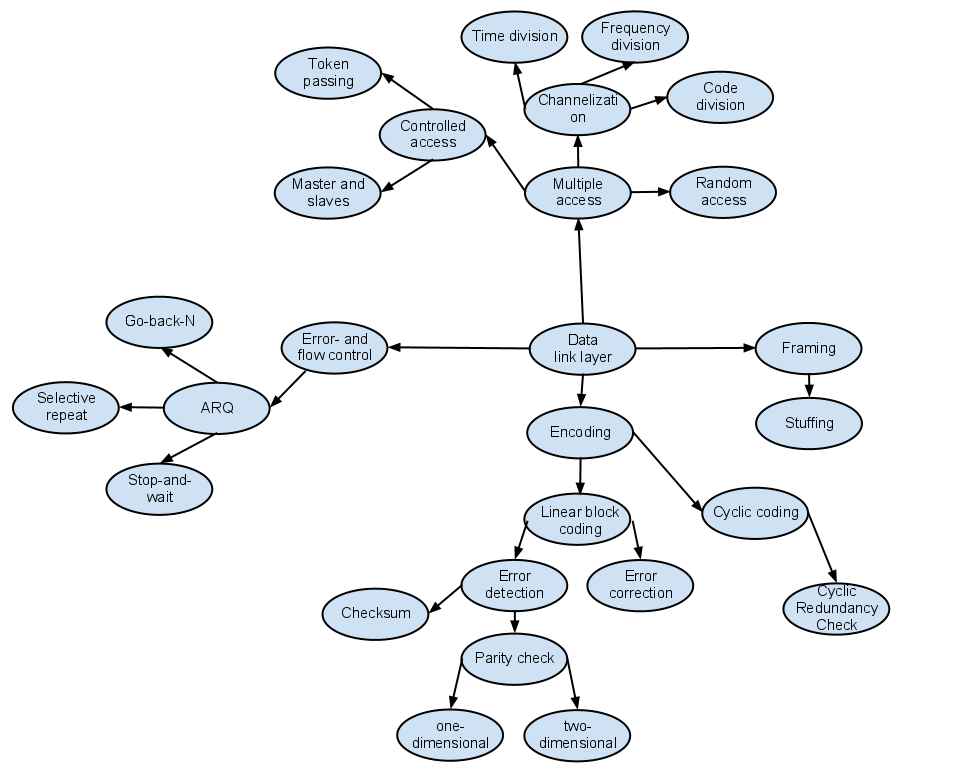
\includegraphics[scale=0.4,trim=0 0 0 0]{dll_bobler.png}%trim=l b r t
	\caption{Things to consider concerning data link layer}
	\label{fig:dll_bobler}
	\end{center}
\end{figure}

\subsection{Encoding}
First thing to consider is the encoding of signals. Since there are sixteen
different DTMF combinations, each tone can carry four bits.

The only type of error to consider is the situation where a tone is
misinterpreted, which leads to a four bit burst error. Therefore the system
should be designed specifically to detect errors of this type. Since the media
is considered to be very noisy, transmissions should also be kept as short as
possible.

A two dimensional parity check will be able to detect burst errors of the
proposed size, so this is the choice. Implementing the parity check as a
four-by-four matrix will make it possible to transfer two bytes with a frame of
three bytes.

Example: We want to transmit the two bytes 0011 0101 and 0101 1110. The data
link layer puts these in a four by four matrix and calculates the parity bits by
adding the rows and columns:

\begin{table}[htb]
	\begin{center}
	\begin{tabular}{c|c}
	0011 & 0 \\
	0101 & 0 \\
	0101 & 0 \\
	1110 & 1 \\
	\hline
	1101 & \\
	\end{tabular}
	\end{center}
	\caption{Two-dimensional parity check}
	\label{tab:two_dimensional_parity_check}
\end{table}

Instead of as normally done to increase the size of each row by one to contain
the parity bit, the parity bits are transmitted together as a redundant byte. In
the case of this example the transmission would be:

\begin{table}[htb]
	\begin{center}
	\begin{tabular}{c|c|c|c|c|c}
	0011 & 0101 & 0101 & 1110 & 0001 & 1101 \\
	\end{tabular}
	\end{center}
	\caption{Bytes to be transmitted}
	\label{tab:bytes_to_be_transmitted}
\end{table}

Each four bit nipple is now transmitted an a DTMF-tone. Should one of the tones
be misinterpreted, the receiving data link layer would get a mismatch of the
parity bits for example:

\begin{table}[htb]
	\begin{center}
	\begin{tabular}{c|c}
	0011 & 0 \\
	0101 & 0 \\
	0000 & 0 \\
	1110 & 1 \\
	\hline
	1000 & \\
	\end{tabular}
	\end{center}
	\caption{Failed parity check}
	\label{tab:failed_parity_check}
\end{table}

This will lead to the frame being discarded. Though in some cases it will be
possible to correct the error and find the original nibble, this is not
recommended, since more than one tone might be corrupted. Errors in the
redundant byte will also lead to the discarding of the transmission.

\subsection{Flow control}
The next thing to consider is flow control. Since the DTMF-system
cannot be used as full-duplex, piggybacking is impossible. This means that at
some point the receiver must reply. This reply will also be of six-tones, and
therefore it might as well contain information about witch frames to resend. In
other words a selective repeat system is preferred

To introduce a selective repeat system, additional redundancy is needed.

By using three bits for the sequence number, redundancy is kept as low as
possible while still benefiting from pipelining. The sender transmits eight
frames (fourty eight tones) and then waits for the receiver to reply with one
frame (six tones).

\subsection{Framing}
It is presumed that the physical layer will provide a starting point for each
transmission. If this is not the case,
additional flags will be needed in between the frames, again leading to the need
of stuffing.

Next thing to consider is multipoint. There are three options: A token
network, a time division network or a code division network. Time division
requires a level of timing the interface layer is unable to deliver.
Code division leads to the need for larger frames or if implemented with the
proposed frame size, a lot of unused frames in a small network. This leaves us
with a token passing network, so this is the choice.

Three bits will control the addressing, all identifying the receiver, since info
about sender is not needed at this level. Thereby the protocol allows networks
of up to eight stations.

The selective repeat system and the token network introduces the need for different frame types.
The type field will consist of two bits, at the same time controlling
the token and indicating frame types. Rules must be implemented to keep the token circulating.

\begin{table}[htb]
	\begin{center}
	\begin{tabular}{|c|ll|}
		\hline
		00 & Has no token & Reply from receiver \\
		\hline
		01 & Has no token & Passes token to addressed station \\
		\hline
		10 & Has token & Accepts token from addressed station \\
		\hline
		11 & Has token & Data frame for addressed station \\
		\hline
	\end{tabular}
	\end{center}
	\caption{Protocol for type field}
	\label{tab:protocol_for_type_field}
\end{table}

Reply frames has type 00 and sequence number 111 (to prevent legal 0:0:0
frames). Each bit of the data byte corresponds to a sequence number and has
value 1 for accepted and 0 for resend.

Token passing is controlled by the backbone architecture of the system and is
implemented in the data link layer. When the token is offered,
there is a window of response time, wherein the station must reply by accepting
the token. If there are no reply during the window, the token is offered to the
next station. 

The backbone has a routine for asking the data link layer whether
it has the token or not. If there are data to send, this is initialized by the
backbone, else the token is passed to the next station. These functionalities
are implemented as public methods in the data link layer.

This leads to the following format of a frame: 

\begin{table}[htb]
	\begin{center}
	\begin{tabular}{|ccc|c|c|}
		\hline
		type (2 bits) & address (3 bits) & sequence (3 bits) & data (8 bits) & parity
		(8 bits)  \\
		\hline
	\end{tabular}
	\end{center}
	\caption{Final frame format}
	\label{tab:final_frame_format}
\end{table}
\section{Transport layer protocol}
In the OSI model, the session and transport layers handle process-to-process sessions (chiefly used when a more permanent connection is required for synchronous transfer, for example) and communication, respectively. When initially exploring ideas for this networking protocol, one wish was that it should be able to serve more than just one application at a time. This brings a need for such process-to-process delivery that the transport layer protocols provide. In this section a transport layer protocol design is described.

\subsection{Speed versus reliability}
A dilemma, when formulating how the transport layer should function, is that as high as possible speed is desired. On the other hand, one must remember, that we wish to make it as painless as possible for the user application to use the connection.\marginnote{Ref til ''Ideer til hvad projektet skal omhandle''-dokumentet} On this layer, the underlying layers (the data link- and physical layers) are not considered to the extent possible. An exception is made, though, as this transport layer protocol is a part of a system, which will not be used on any other medium than sound.

A UDP\footnote{User datagram protocol}\nomenclature{UDP}{User datagram protocol}-like protocol design would no doubt be one of the best ways to achieve high transfer speeds. The UDP protocol provides a connectionless service, where datagrams are sent and then forgotten. That way the receiver does not have to spend bandwidth to acknowledge successful reception. Additionally, the header size of a datagram is quite small, as there is no error- or flow control. There is not any sequence number either, so datagrams are sent without any way of knowing whether they are received in-order.

Using a TCP\footnote{Transmission control protocol}\nomenclature{TCP}{Transmission control protocol} inspired protocol, instead of UDP, would enable the transport layer to provide a much more reliable service. Now, with the TCP protocol, flow- and error control is added, as well as congestion control. Every packet is assigned a sequence number, ensuring they are passed on to the server application correctly, by the receiving transport layer protocol. Every packet is also acknowledged by the receiver, if it is successfully recorded. If not, the sender re-sends them. All these things combined makes TCP a lot more reliable, but it also increases it's header size to around three times the size of the UDP header. Especially if one is not sending a lot of data in each packet, the header can take up a large percentage of the combined (header plus data) package size.

The application making use of the transport layer protocol, should not have to worry about data loss. Therefore a certain level of error control, as well as sequencing, is requested. Since the transfer in general is not very fast in the combined system\marginnote{Needs ref}, flow control can safely be ignored in this design. Congestion control is not needed either, as only two nodes will communicate with each other at a time, across a half-duplex\marginnote{Needs ref} line.

Thus, the transport protocol design will contain a mixture of the properties described above, and following specifications can be formulated: The protocol should
\begin{itemize}
  \item provide reliable delivery up to a maximum number of retransmissions (i.e. avoid stale signaling messages)
  \item provide in-order delivery. 
  \item have low overhead and high performance. 
  %\item transport should provide a keep-alive mechanism. 
  \item provide error detection. 
\end{itemize}

A more detailed portrayal of each feature, and how they are to be used, will follow in the next sections.

\subsection{Addressing processes}
The data link layer in our model takes care of the node-to-node delivery, where each node has an address. This address is, however, not at all useful to the transport layer \textit{after} a node's data link layer has received data and passed it on. Thus, we need a different addressing method to distinguish signaling processes from each other: A port number.\footnote{Port number, in this text, is separate from the port number normally associated with a process when it \textit{binds} via some kind of Internet socket. Still, the term is used, as it's purpose is identical to the ''normal'' port number.}

The port number assigned to a certain server\marginnote{Define server and client as used here} application must be known to the client before it sends anything. That is the only way the local process will know where to send data. Here, we select the port number to be eight bits long. This reasoning behind this choice is, that we will not at all be able to serve more than a couple of applications at a time, at the most. Add to that, that we wish to keep a minimal overhead size (a higher port number would add more bits to the header), as we don't have a lot of bandwidth available to begin with.

A number of port addresses (0-19)\marginnote{subject to change} are going to be reserved for special messages and are therefore not available for applications to use. Refer to Table \ref{tab:trans_well_known} for a list of reserved ports and their uses.
\begin{table}[htb]
 \centering
 \begin{tabular}{cl}
  \textit{Port} & \textit{Description}\\
  \midrule
  1 & Does something?\\
  \midrule
  4 & Not sure what this does\\
  \midrule
  17 & Does something else
 \end{tabular}
 \caption{Well-known ports used by the transport layer protocol}
 \label{tab:trans_well_known}
\end{table}

\subsection{Sequencing}
To\marginnote{Not entirely done from here on} make sure the receiver passes on data to the above layer correctly, sequence numbering is introduced. Every packet that is sent will have a number attached, to help the receiving end order segments accurately. The sequence number is $8$ bits long. A segment will also have an $8$ bit acknowledgment number, which is closely related to the sequence number, as we shall see.

When a connection is initiated, a random number between $0$ and $2^8-1$ is selected. Each transmitter increments this number before sending a segment, except in a few special cases. 

The acknowledgment number indicates to the transmitting party the last in-sequence packet the receiver has received. %%

\subsection{Error control}
Header is always checksummed. If the \texttt{CHK} flag bit is set, a checksum is calculated for the whole datagram. This gives

\subsection{Datagram}
From the application, the transport layer protocol expects to just receive a stream of bytes. The order in which the bytes are received is significant, but the data they contain is not. When received, the bytes will be packed into datagrams...
\begin{table}[htb]
 \centering
 \begin{tabular*}{0.70\textwidth}{@{\extracolsep{\fill}}|c|c|c|c|c|c|c|c|c|c|c|c|c|c|c|c|}
  %
  \multicolumn{1}{c}{\texttt{0}} & \multicolumn{1}{c}{\texttt{1}} & \multicolumn{1}{c}{\texttt{2}} & \multicolumn{1}{c}{\texttt{3}} & 
  \multicolumn{1}{c}{\texttt{4}} & \multicolumn{1}{c}{\texttt{5}} & \multicolumn{1}{c}{\texttt{7}} & \multicolumn{1}{c}{\texttt{8}} & 
  \multicolumn{1}{c}{\texttt{9}} & \multicolumn{7}{r}{\texttt{15}}\\
  \hline
  %
  \multicolumn{8}{|c|}{   \multirow{3}{*}{Source port addr.}   } & \multicolumn{8}{c                  |}{   \multirow{3}{*}{Destination port addr.}   }\\
  \multicolumn{8}{|c|}{                                        } & \multicolumn{8}{c                  |}{                                             }\\
  \multicolumn{8}{|c|}{                                        } & \multicolumn{8}{p{0.312\textwidth} |}{                                             }\\
  \hline                                                                           % ^ above width is to acquire symmetry
  %
  \texttt{S} & \texttt{A} & \texttt{C} & \texttt{R} & \texttt{F} & \texttt{ } & \texttt{ } & \texttt{ } & \texttt{ } & \texttt{ } & \texttt{ } & \texttt{ } & 
  \multicolumn{4}{c|}{     \multirow{3}{*}{HLEN}     }\\
  \texttt{Y} & \texttt{C} & \texttt{H} & \texttt{S} & \texttt{I} & \texttt{0} & \texttt{0} & \texttt{0} & \texttt{0} & \texttt{0} & \texttt{0} & \texttt{0} & 
  \multicolumn{4}{c|}{                               }\\
  \texttt{N} & \texttt{K} & \texttt{K} & \texttt{T} & \texttt{N} & \texttt{ } & \texttt{ } & \texttt{ } & \texttt{ } & \texttt{ } & \texttt{ } & \texttt{ } & 
  \multicolumn{4}{c|}{                               }\\
  \hline
  %
  \multicolumn{8}{|c|}{    \multirow{3}{*}{Sequence number}    } & \multicolumn{8}{c|}{     \multirow{3}{*}{Acknowledgment number}        }\\
  \multicolumn{8}{|c|}{                                        } & \multicolumn{8}{c|}{                                                   }\\
  \multicolumn{8}{|c|}{                                        } & \multicolumn{8}{c|}{                                                   }\\
  \hline
  %
  \multicolumn{16}{|c|}{           \multirow{3}{*}{Checksum}           }\\
  \multicolumn{16}{|c|}{                                               }\\
  \multicolumn{16}{|c|}{                                               }\\
  \hline
  %
 \end{tabular*}
 \caption{Transport layer datagram header}
 \label{tab:trans_datagram_header}
\end{table}

\subsection{Operation}
connection-oriented, handshake, data push

%================= OLD =================
%
%\begin{table}[htb]
% \centering
% \begin{tabular}{rcccc}
%  \textit{Bits} & 0-7 & 8-15 & 16-23 & 24-255\\
%  \midrule
%   & Source port & Dest. port & Length & Data
% \end{tabular}
% \caption{Transport layer datagram format}
% \label{tab:trans_datagram_format}
%\end{table}
%
%
%
%\subsection{Operation}
%Much like the UDP\nomenclature{UDP}{User datagram protocol} this transport layer protocol provides a connectionless service, meaning packets are sent without having to first establish a connection. Also they are sent without sequence numbers, though in our case this is not a problem. This protocol will only be used on a half-duplex line, and there is no routing from one network to another: The packets can only go one way, and there is only one packet on the line at a time, thus packets cannot be ''out of order''.
%
%In this protocol, no flow or error control is incorporated.\marginnote{If needed we can implement error or flow ctrl anyway} This is mainly due to the reason that the data link layer and transport layer communicate directly, and not across networks where another protocol might provide an unreliable service (as with the IP\footnote{Internet protocol}\nomenclature{IP}{Internet protocol} which is provides \textit{best effort} delivery). With no error or flow control we save yet some more overhead space.
%
%With each application getting a different port number, the transport layer protocol being developed provides application multiplexing. That is, more than one application can use the protocol at the same time on each node. 
%
%
%%%%%%%%%%%%%%%%%%%%%%%%%%%%%%%%%%%%%%%%%%%%%%%%%%%%%%%%%%%%%%%%%%%%%%%%%%%%%%%%
% Kims ''thinking'' ^o~
%%%%%%%%%%%%%%%%%%%%%%%%%%%%%%%%%%%%%%%%%%%%%%%%%%%%%%%%%%%%%%%%%%%%%%%%%%%%%%%%
%
%error control
%multiplexing
%well known ports (for ''control'')
%datagrams (variable length, but with max.)
%
%As a low overhead is preferred, it is natural to look to the UDP\footnote{User datagram protocol}\nomenclature{UDP}{User datagram protocol}. The UDP transport layer protocol provides a connectionless service and unreliable service.
%
%Also they are sent without sequence numbers, though in our case this is not a problem. This protocol will only be used on a half-duplex line, and there is no routing from one network to another: The packets can only go one way, and there is only one packet on the line at a time, thus packets cannot be ''out of order''.
%
%
% IN:
% ----
% * Byte-array
% * Source port number       \
% * Destination port number   \_ (or do we know this already?)
%
% OUT:
% ----
% HEADER                        DATA
% 
%
% ''session''-delen er lidt ude i kulden? connection oriented transport layer protokol kan det, vi gerne vil?
%
% sekvensering
% process-process
% process ID (PID) / ''port'' number
% (de)multiplexing
% in/out queue-buffer (one for each port)
%   overflow
%   unreachable/queue non-existant
% reserved ports for system messages?
% flow control, we don't need (?)
% unrealiable sending ?
% connectionless service ?
% congestion, we dont care?
%
%
% socket address = ''data link layer''-address + port number
%
%
%variabel datal�ngde, sekvensnummer, sessionID,modtager, afsender,flag
%
\chapter{Implementation}
How was it made?

\begin{itemize}
\item each layer
\item backbone
\item test class
\item application to use with our network
\end{itemize}
\section{Data link layer}
The data link layer is implemented in the form of two classes. The DataLinkLayer
object is instantiated by the backbone and the Frame and Datagram objects are
instantiated by the DataLinkLayer and destructed by it when processed.

\begin{figure}[htb]
	\begin{center}
	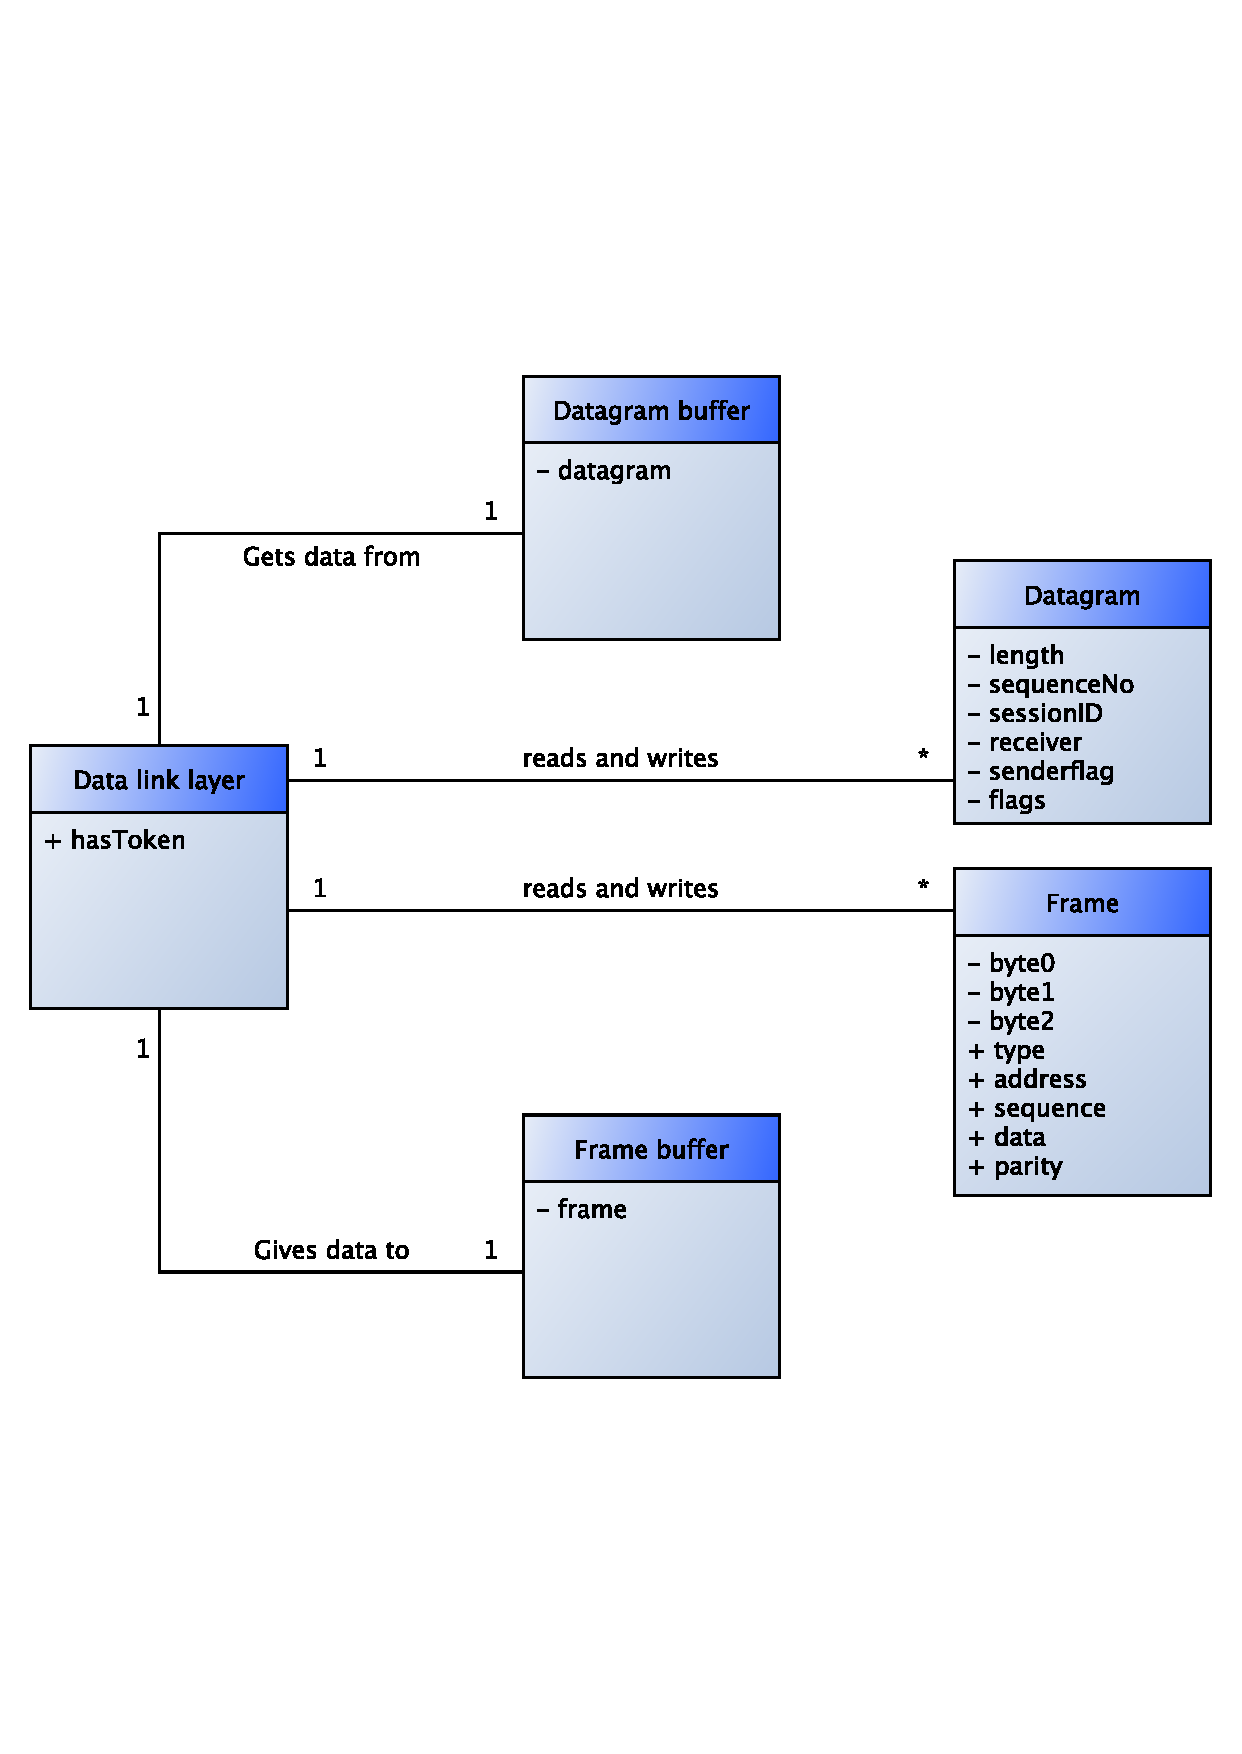
\includegraphics[scale=0.5,trim=0 0 0 0]{dll_class_diagram.pdf}
	\caption{Class diagram for data link layer (incomplete)}
	\label{fig:class_diag_for_datalink}	
	\end{center}
\end{figure}

The methods of the classes are developed to realize the flowchart of the data
link layer. Decisions on whether to implement a method in one class or another
is done using the expert pattern.

\begin{figure}[htb]
	\begin{center}
	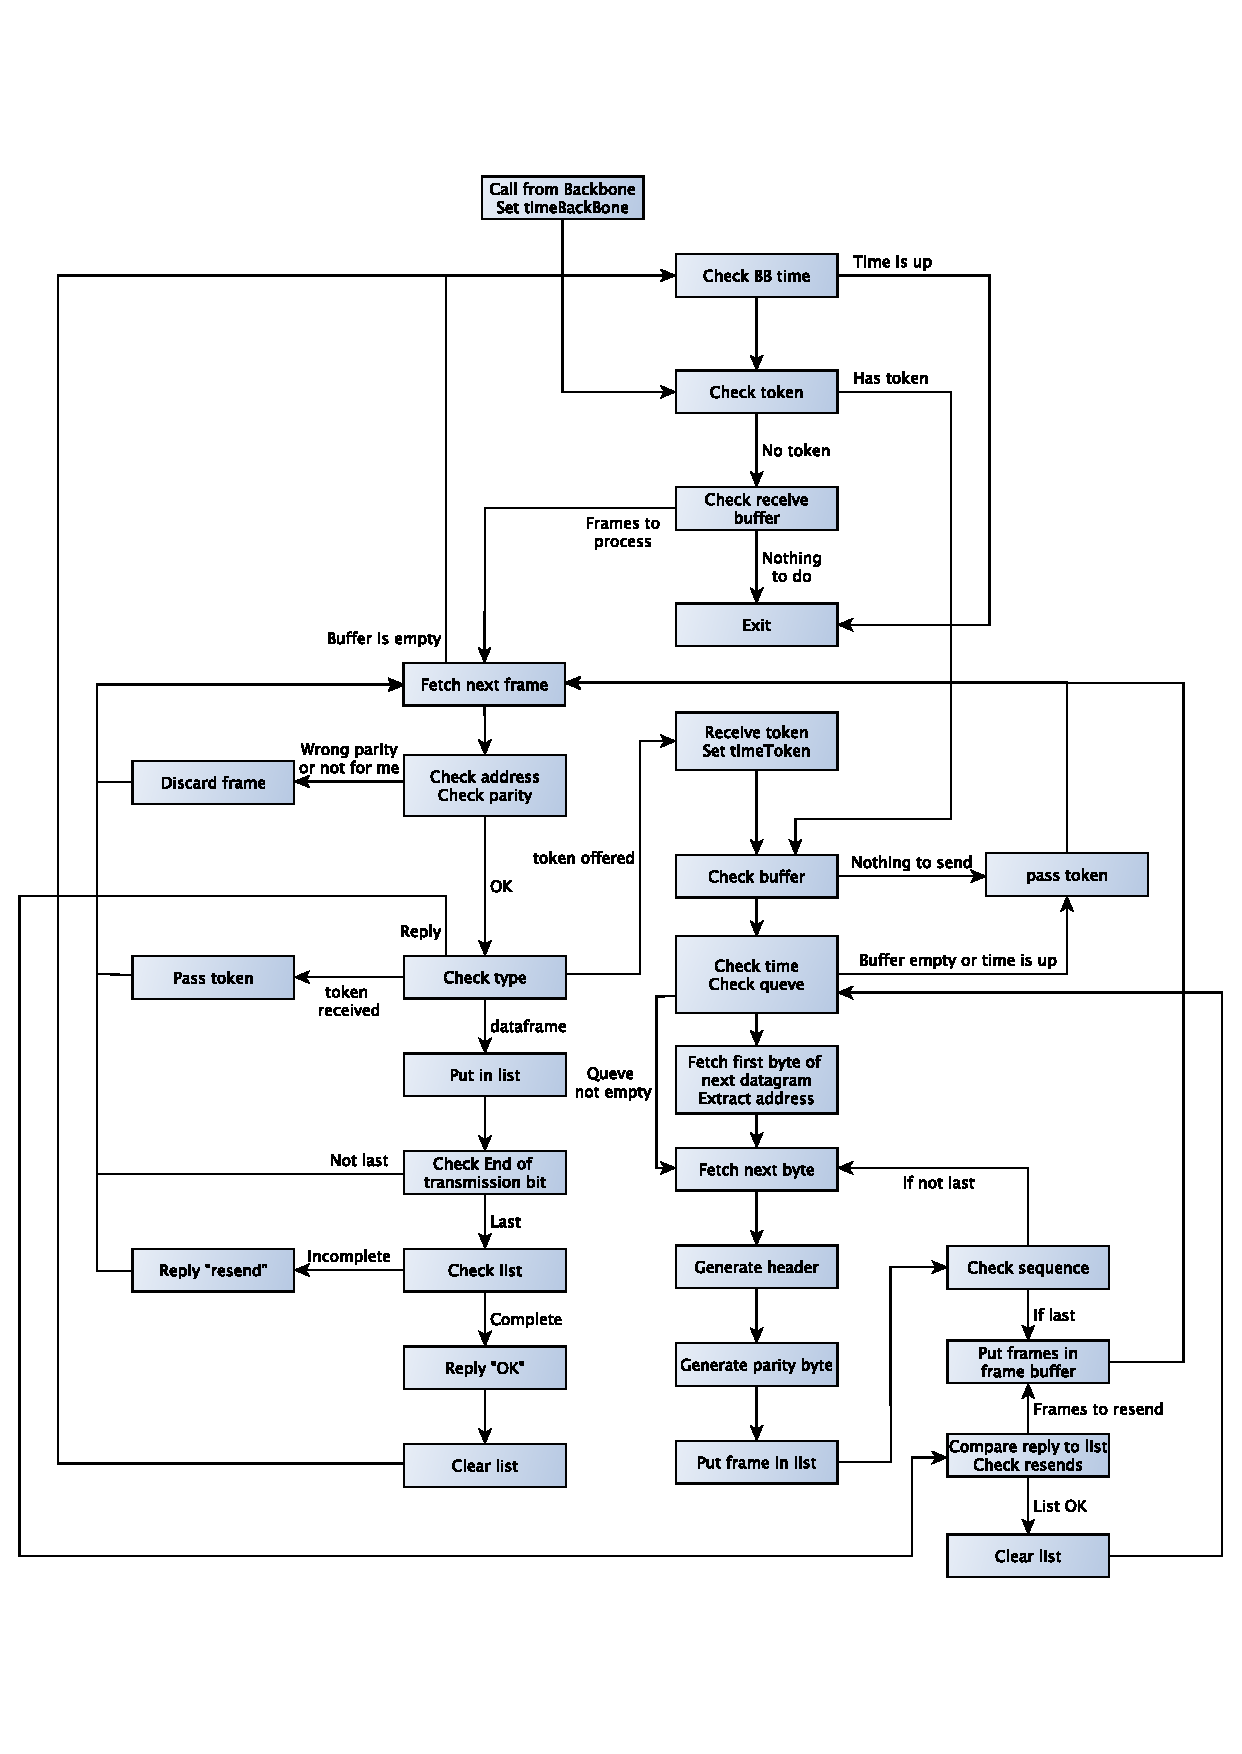
\includegraphics[scale=0.5,trim=0 0 0 0]{dll_flowchart.pdf}
	\caption{Flowchart for data link layer}
	\label{fig:flowchart_for_datalink}	
	\end{center}
\end{figure}
\section{Transport layer}
Nemlig
%
\chapter{Experiments}\label{chap:experiments}
Throughout development a lot of testing have been done towards debugging the program. However this chapter is only concerned about tests of the systems conditions. Tests beformed to get a knowlegde of the layers abilities concerning performance and reliability. Thus it will be possible to gain an overwiev of the application. The results of souch tests will ofcourse depend the used computers ability, standard laptops were used. 


This chapter descripes the perfomed tests and the results gained.






\section{Test Function Documentation}
To be able to make easy and similar tests for all the layers, it was decided that we developed a function to make test. The function is able to send data to a layer as if it was the neighbouring layers. Thus the function makes it possible to give input to a layer and check the output.

\begin{figure}[htb]
	\begin{center}
	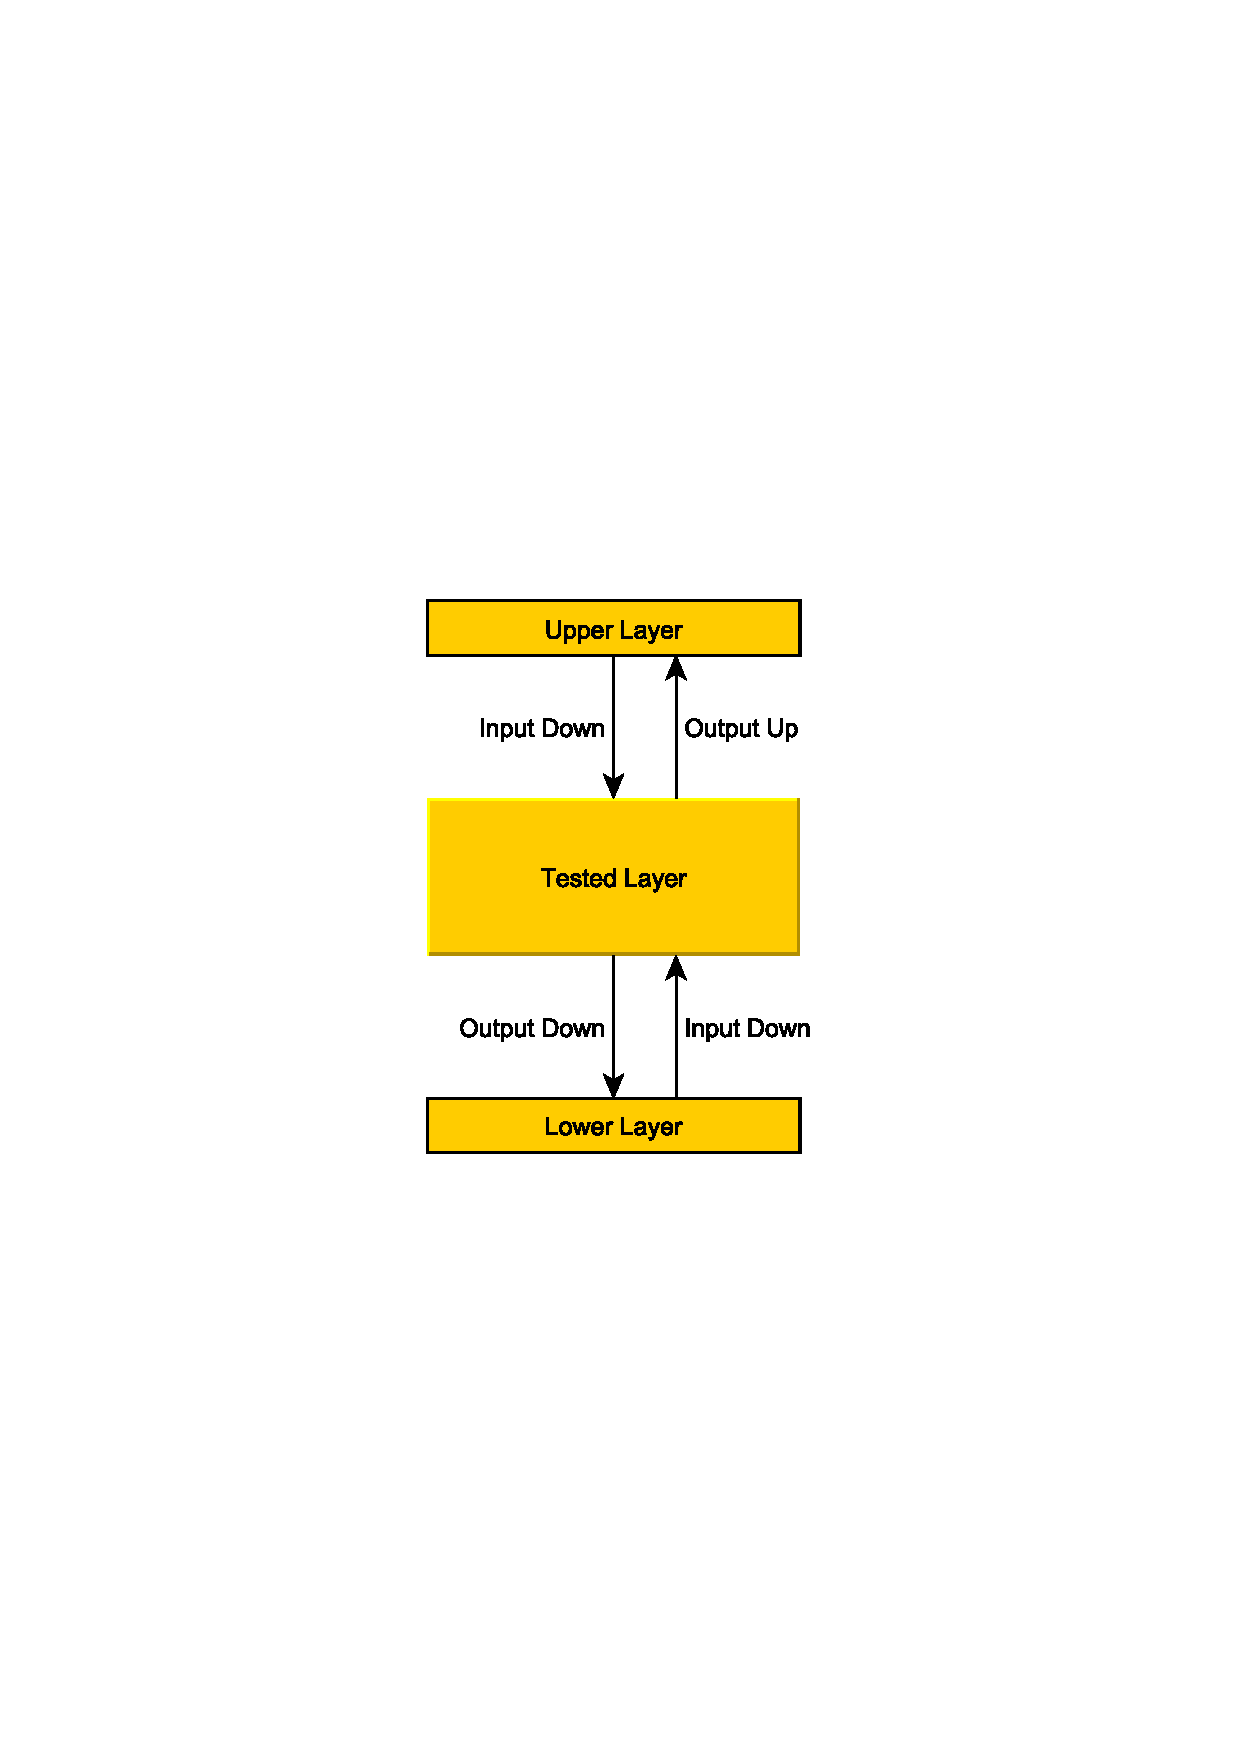
\includegraphics[scale=0.5,trim=0 0 0 0]{Layer_inputoutput.pdf}
	\caption{Substituting surrounding layers (incomplete)}
	\label{fig:Layer_inputoutput}	
	\end{center}
\end{figure}

Use of Input Output functions
To make it easy to change and manipulate the input and output, is it defined in .dat documents. Therefore the program doesn't have to be changed for different input, and the output can be easily extracted for further analysis. Ifstream and Ofstream are used to read and write from the documents. In the 
BOOST buffer
As the boost buffer is used as communication between the layers, is it also used as the test functions mean of communication with the layer tested. There are defined four buffers, two for input and two for output.
Use of test function
In the beginning one simply includes the layer and in the function sets the name of the layer. It's is possible to change the defined names for the .dat files. The boost buffers are defined for the layer, so with this setup it's just running the program.

\begin{figure}[htb]
	\begin{center}
	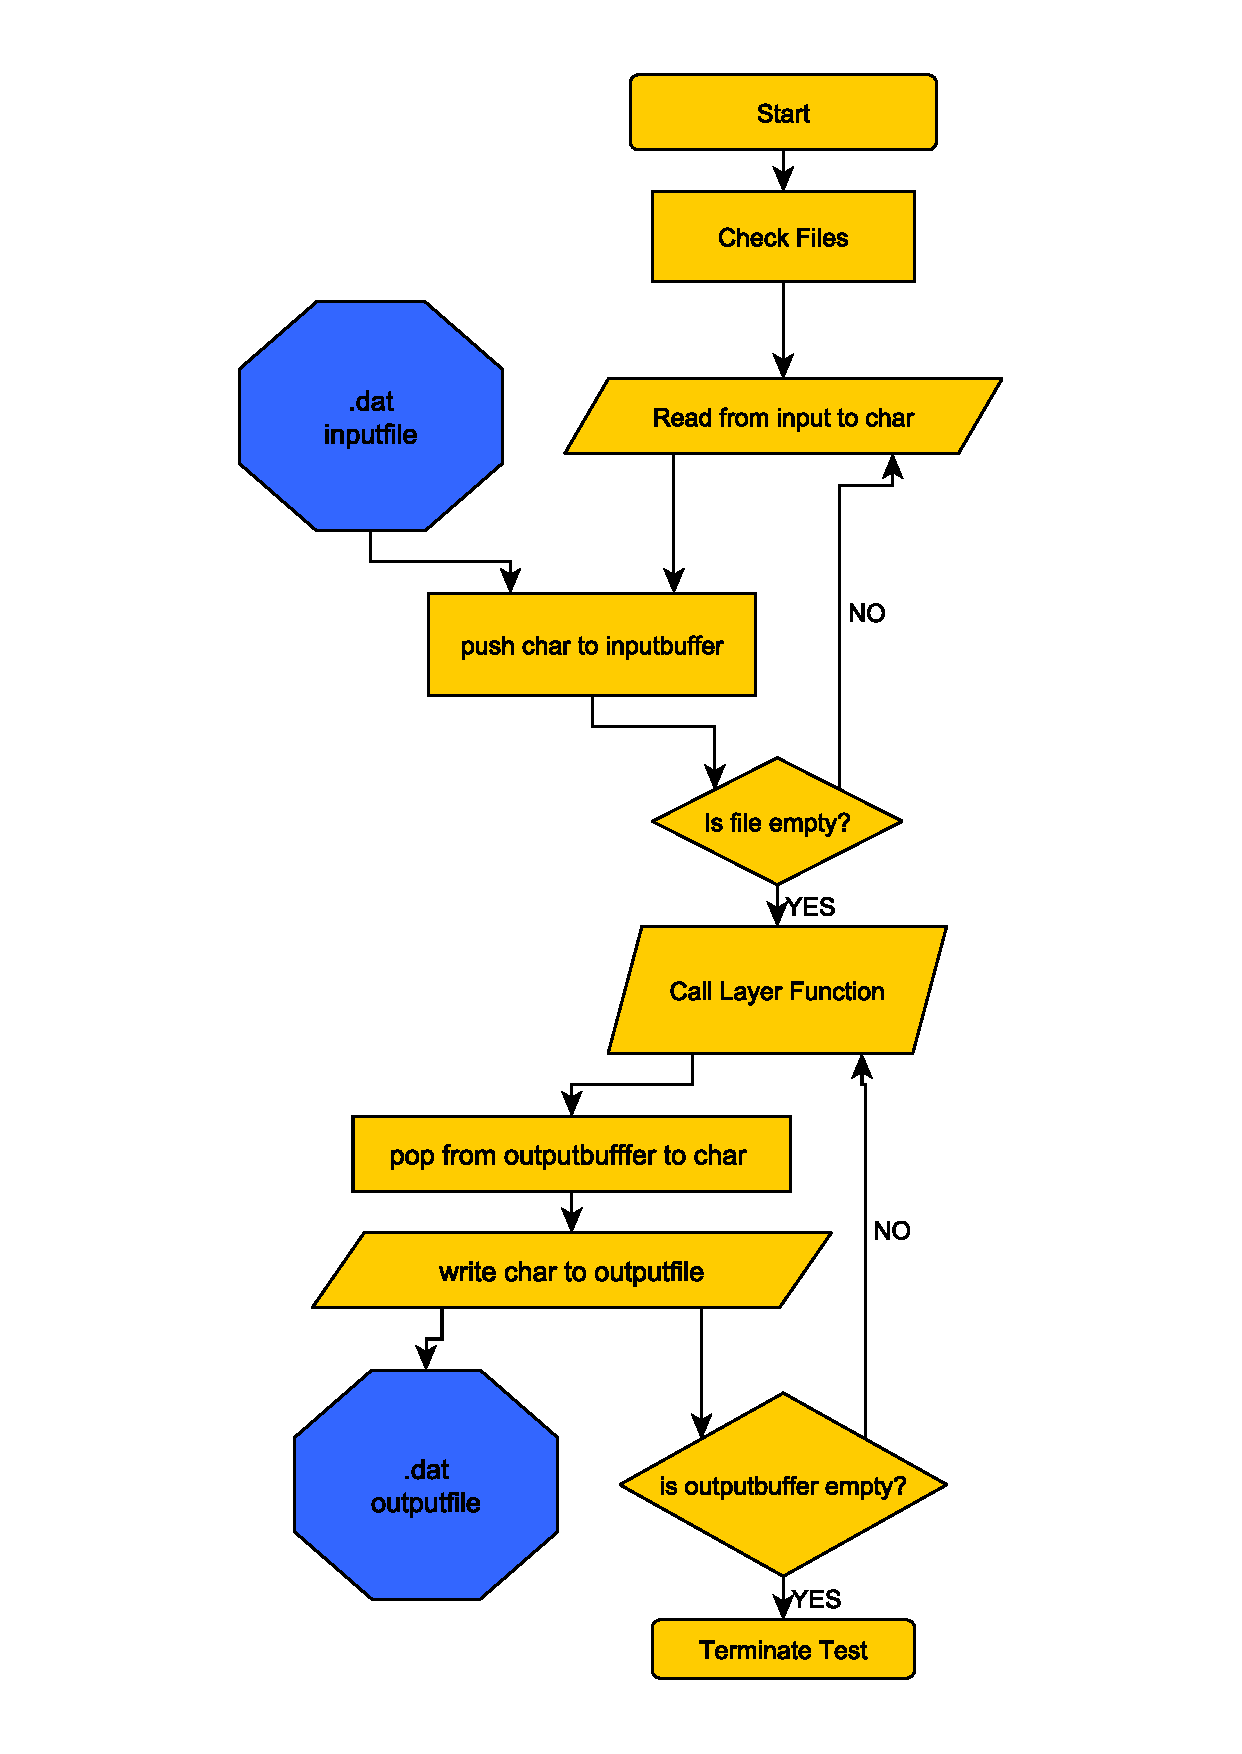
\includegraphics[scale=0.5,trim=0 0 0 0]{TestFlowchart.pdf}
	\caption{Flowchart for test function (incomplete)}
	\label{fig:TestFlowchart}	
	\end{center}
\end{figure}


%
\chapter{Discussion}\label{chap:discussion}
The main idea about implementing the generic protocol stack has been to find an approach
where each member of the team was able to dig deeply into the essence of the
professions while still making it easy to compile the different parts of the
project into a coherent solution.

The chosen approach was to define clean interfaces between the software layers
in the form of predefined buffers. This has proven to be a powerful tool, since
each layer has been debugged and tested individually. Also a lot of potential
problems about the overall flow- and software control was avoided, since all
methods and loops were connected in the backbone program.

The architecture has provided a certainty of maximum reuse of
code and have efficiently avoided unnecessary coupling in the software. Because
of the bold ambition to create a compiled library for other developers to use, the problem reached a
size, where efficient programming was imperative. Time was also an issue and
again the procedure has proven most beneficial because each team member has been
able to work and test independent of the others, thereby avoiding time wasted in
waiting for other parts to finish.

The respective layers have been developed using an iterative approach, where
the individual team member has worked on his part and then presented it to the rest
of the group either by internal documentation on the project wiki, input to the
report, demonstration programs or by giving short lectures in the subject. This
way the team has been able to work efficiently while still pulling together.

The distribution of team roles has been a challenge, mostly because it implies a
new way of thinking in behaviour and responsibilities instead of duties and
fields of expertise. It was an informed choice to select the team roles from a
point of learning and not a point of experience. This decision ensured that
all members started on equal feet, but also imbued some difficulties of breaking
old patterns. It has provided some serenity to the work, knowing that one does
not have to be mindful of the entire project, trusting that other team members
will do their part.

Professionally the project has given hands on experience of the OSI layers
taught in data communication and a much greater understanding of the material.
Developing a large software system leads to considering the UML language and
advantages of object oriented programming, supporting the lectures in software
development. Since all members of the team have contributed to the source code,
a much greater experience in C++ programming has been obtained. Finally the
analysis of the problem and to some extend implementing the tone detection
system has lead to a greater understanding of digital signal processing.
\chapter{Conclusion}\label{chap:conclusion}
Questions to be answered:

To what extend was it possible to make an API that implements a DTMF based
network?
How did the system perform during test? 
Are there things that should be testet further?

To what extend does the physical layer work? 
The physical layer works like a charm, according to table \ref{tab:exp_phys_speaker} a bit rate around $110\sfrac{bit}{s}$ can be reached without compromising the reliability too much. Several optimisation possibilities are available, but not needed as stability is not an issue.

  To what extend does the data link layer work? 
The data link layer is able to process a packet and enclose it in a sequence of
frames to be sent. It is also able to receive frames and to process them into at
packet to be delivered to the transport layer. The data link layer is also able
to control a token based network in a way that allows collision free half duplex
communication. 

  How did the data link layer perform during test? The data link
layer performed well under test and handles communication with up to sixty
percent errors, though this amount of errors makes it very slow. With more than
sixty percent errors all time goes into contol talk and almost no frames are
transmitted.

  What could make it even better?
If it is possible to find a way of using a sliding window instead of the eight
byte list currently implemented. There is currently a lot of transmission time
being wasted in sending lists shorter than eight entries. Other changes could be
considered to handle cases where a crucial frame is lost. For example the case
where a reply is lost which results in some waiting time and the entire list
being resend.

To what extend does the transport layer work? 
How did the transport layer perform during test?
What could make it even better?

To what extend does the API layer work? 
How did the API layer perform during test?
What could make it even better?

To what extend does the Backbone work? 
The backbone class works as expected. It is able to dispatch work to the correct layer objects, based on the state of the internal buffers and layers.
How did the backbone perform during test?
The backbone has not been tested, as it is meaningless to test it without the actual layers combined. Since the final assembly has not been completed at the time of writing, any backbone tests are impossible. However the backbone has been debugged and everything seems to be functioning properly.
What could make it even better?
The input and output stacks could have their own backbone thread, inorder to simplify the logic of which buffer to check.
The communication to the physical layer could be handled through an actual queue with a mutex on the last element, instead of a ringbuffer. The logic to detect whether the network layer and datalink layer have room to perform their actions needs to be improved.


How did the test function work?
When used the test function worked as planned, and where adapted to the tested layer. 
How much was it used?
Some used the test function to a great exstent, unfortunaly not all tests were performed with the test function. This could have been solved by being more clear from start about how the layers were to be tested . 

To make the test function more efficient more options for testing could have been added.

% 
% References
\clearpage
\nocite{*} % Inkluderer alle poster i bibl.bib-filen (dvs. kun skriv litteratur ind vi rent faktisk har brugt)
\printbibliography\addcontentsline{toc}{chapter}{Bibliography}
%
% Appendix
\appendix %all sections below are numbered A, B, C,...
\chapter{PortAudio}\label{chap:lib}\label{app:portaudio}
As this project requires the usage of the sound card in a computer some interface is needed. A quick search on Google resulted in a countless number of possibilities for interfacing a C++ program with the sound card of a computer. The team decided on a set of requirements which the interface had to provide. Requirements are listed below:

\begin{itemize}
\item Easy-to-use application programming interface.
\item Cross platform.
\item Access to raw sample data.
\item Variable sample speed.
\item Support multiple streams.
\end{itemize}

The surface of several interfaces was scratched to see what they had to offer. Some of the possibilities are listed below:

\begin{description}
\item[RT Audio\footnote{}] was crap...
\footnotetext{\url{http://www.music.mcgill.ca/~gary/rtaudio/}}

\item[QT Multimedia\footnote{}] is developed by Nokia, and is a good suggestion as it comply with the requirements. The disadvantage is that core files from QT itself is needed which result in increased size of the developed software. Not that the size is specified as a requirement of the project itself but it also result in a superior complexity of the developed software itself, so QT Multimedia was discarded.
\footnotetext{\url{http://doc.qt.nokia.com/latest/qtmultimedia.html}}

\item[PortAudio\footnote{}] was finally chosen as the lowermost component of the software as it comply with the requirements mentioned above.  The reason for this final decision was based on the simplicity of the usage of PortAudio. Beside this point it is extremely adaptable which make it possible to use in a wide range of applications. A block diagram can be seen in figure \ref{fig:app_portaudio}.

\begin{figure}[htb]
	\begin{center}
	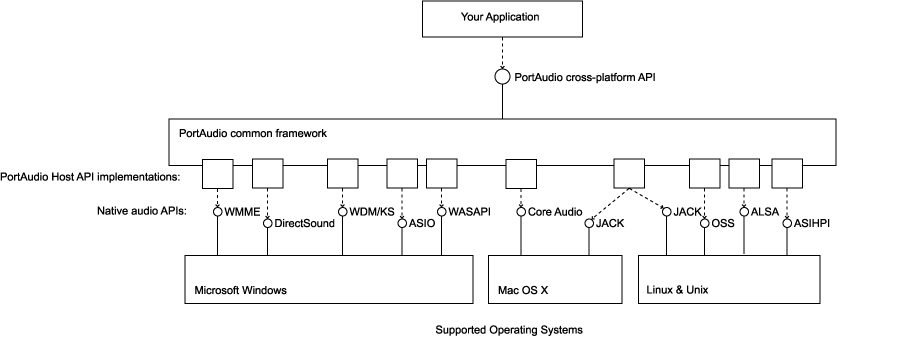
\includegraphics[scale=0.4,trim=0 0 0 0]{portaudio_architecture.png}%trim=l b r t
	\caption{This is an overview of the PortAudio interface.}
	\label{fig:app_portaudio}
	\end{center}
\end{figure}

\footnotetext{\url{http://www.portaudio.com/}}
\end{description}%not sure if this should be here at all, yet
%
\end{document}
